%% Q1
Higher education aims at independent thinking, inquiry (probing), creativity and ``thinking out of the box''. Mere \textbf{preparation for examinations} is the \emph{least desirable} outcome: it encourages rote learning.

%% Q2
An effective teacher combines \textbf{mastery of the subject (1)}, \textbf{effective oral communication (2)} and \textbf{the respect of students (4)}. Being respected by society's leaders (5) and a pleasant presence (3) are not essential qualities of teaching. The answer is 1, 2, 4.

%% Q3
\textbf{Field study} puts learners in real, open-ended situations where they observe, explore, question and produce original ideas, which develops creativity.
\why{Lecture and demonstration are teacher-centred; self-learning material is structured and convergent.}

%% Q4
\textbf{Formative assessment} takes place \emph{during} the teaching--learning process to monitor progress and provide feedback (assessment \emph{for} learning). Summative assessment comes at the end.

%% Q5
\textbf{Classroom discussion} involves learners actively: they express, question, listen and build on others' ideas. This deepens understanding far more than passively receiving notes or explanations.

%% Q6
In \textbf{constructivism} (Piaget, Vygotsky, Bruner) the learner is an active \textbf{explorer} who constructs knowledge through exploration and experience. The learner is not a passive responder.

%% Q7
When every unit of the population has an \textbf{equal (and independent) chance} of selection, the method is \textbf{random (probability) sampling}.

%% Q8
Studying the future of an institution requires the considered views of many stakeholders and experts. A \textbf{questionnaire} can collect these systematically from a large, spread-out group; futures studies such as the \emph{Delphi technique} use successive rounds of questionnaires to build consensus about the future.

%% Q9
A research hypothesis is a specific, testable statement. It can be declarative, null or directional, but it \textbf{cannot be in question form}. (A question is a research \emph{question}, not a hypothesis.)

%% Q10
Presenting someone else's text without acknowledging the source is \textbf{plagiarism}.

%% Q11
The logical research sequence: \textbf{identify the problem $\rightarrow$ select the sample $\rightarrow$ develop tools $\rightarrow$ collect data $\rightarrow$ analyse data}, which is option (D).
\tip{Some texts place tool development before sampling. Either way, the problem comes first and data analysis comes after data collection.}

%% Q12
\textbf{Action research} (Stephen Corey applied it to education) is carried out by practitioners such as teachers and counsellors to solve \emph{their own immediate problems} systematically and improve practice.

%% Q13 ctx
\textbf{Read the paragraph and answer the Question Nos.~13--18.}\par\smallskip
Adolescence is a period of rapid growth and development bridging childhood and adulthood. Practicing healthy eating behaviour is one of the most important factors to meet the nutritional needs of adolescents. Proper eating behaviours that are learned in early life are maintained in adulthood thus reducing the risk of major chronic diseases. Physical and psychological changes occurring during this period usually significantly influence their dietary behaviours. As teens become more independent, they make more of their own food choices. However, being influenced by a massive amount of factors (biological, social, physical, economic, psychological beliefs and knowledge about food) and changing of lifestyle may affect their dietary choices and eating behaviour, thus making them fail to adhere to healthy eating practices. Peer pressure in colleges leads adolescents to eating non-nutritional foods like pizzas and burgers. Due to irregular college schedules, intake of caffeinated drinks increases and water intake reduces. Poor nutrition can lead to reduced concentration in studies, low stamina, depression or poor posture.

%% Q13
The official key gives \textbf{peer pressure in colleges}: ``Peer pressure in colleges \textbf{leads} adolescents to eating non-nutritional foods like pizzas and burgers.'' This is the direct cause the passage names for giving in to unhealthy foods.

%% Q14
Pizzas, burgers, caffeine and less water are examples. What they add up to is a \textbf{poor nutritional diet}, the general meaning of unhealthy dietary habits.

%% Q15
``\textbf{Poor nutrition} can lead to reduced concentration in studies.'' Poor nutrition means \textbf{not being able to meet nutritional needs}.

%% Q16
Adolescence bridges childhood and adulthood because it is a period of rapid growth, i.e.\ \textbf{physical and psychological changes}.

%% Q17
Dietary behaviour refers to how a person \textbf{makes choices about diet}: what, when and how much to eat (``as teens become more independent, they make more of their own food choices'').

%% Q18
``Proper eating behaviours that are learned in early life are maintained in adulthood, thus reducing the risk of major chronic diseases.'' By the same logic, poor eating in adolescence \textbf{sows the seeds of ill health in adulthood}.

%% Q19
The sender \textbf{encodes}: converts ideas into symbols (words, signs). Decoding and reception are the receiver's functions; feedback is the receiver's response.

%% Q20
In a classroom the teacher speaks to individual students \textbf{(i)} and to the whole class \textbf{(ii)}, and the class or a group responds to the teacher \textbf{(iii)}. The answer is (i), (ii) and (iii).

%% Q21
\textbf{Encryption} converts the content into a code that only the intended recipient (with the key) can read, protecting sensitive e-mail matter.

%% Q22
Communication from a superior to subordinates is \textbf{downward communication}.

%% Q23
Communication through body movements (gestures, postures) is \textbf{gestural} (kinesic) non-verbal communication.

%% Q24
\textbf{Sender $\rightarrow$ Message $\rightarrow$ Receiver $\rightarrow$ Feedback}.

%% Q25
The product is written with its digits reversed:
\[2\times7=14\rightarrow41,\qquad4\times3=12\rightarrow21,\qquad5\times5=25\rightarrow52\]
\[3\times6=18\rightarrow\mathbf{81}\]

%% Q26
A person first \textbf{studies (5)}, then gets \textbf{service} (a job) (2), which brings \textbf{income (3)}, which gives \textbf{status (1)}, and finally \textbf{settlement (4)} in life. The order is 5 $\rightarrow$ 2 $\rightarrow$ 3 $\rightarrow$ 1 $\rightarrow$ 4.

%% Q27
Each term is $n(n-1)$: $1\cdot0=0$, $2\cdot1=2$, $3\cdot2=6$, $4\cdot3=12$, $5\cdot4=\mathbf{20}$, $6\cdot5=30$. (Differences: 2, 4, 6, 8, 10.)

%% Q28
Each letter is replaced by its alphabet position written \emph{in reverse}: N $=14\rightarrow41$, O $=15\rightarrow51$, T $=20\rightarrow02$, giving 415102.
SRP: S $=19\rightarrow91$, R $=18\rightarrow81$, P $=16\rightarrow61$, giving \textbf{918161}.

%% Q29 note
No single consistent rule fits all three given examples. Students should record the official answer and not spend exam time on such items.

%% Q29
The official key gives \textbf{(D) 144}. The first two examples fit $(b+1)^{a-1}$: $(6+1)^{2-1}=7$ and $(2+1)^{4-1}=27$. The third ($7\times3=144$) does not fit that rule, and no rule gives any of the options for $5\times8$ unambiguously. The question is best treated as defective; answer according to the key.

%% Q30
Each term is $n^2(n+1)$ for $n=0,1,2,3,4$: $0$, $1\cdot2=2$, $4\cdot3=12$, $9\cdot4=\mathbf{36}$, $16\cdot5=80$.

%% Q31
The number is the letter's position $+3$: A(1)$+3=4$, F(6)$+3=9$, M(13)$+3=\mathbf{16}$, Q(17)$+3=20$.

%% Q32
The letters advance by 5: C(3), H(8), M(13), \textbf{R(18)}, W(23).

%% Q33 ctx
There are total 400 candidates applying for admission to one of the courses C1, C2, C3, C4 and C5, for study. The given table shows \% number of all 400 candidates admitted to these courses. Based on this table, answer the following questions (33--35):
\begin{center}
\begin{tabular}{lcccccc}\toprule \textbf{Course} & C1 & C2 & C3 & C4 & C5\\\midrule
\textbf{\% admitted} & 15 & 10 & 25 & 30 & 20\\
\textbf{Number} (of 400) & 60 & 40 & 100 & 120 & 80\\\bottomrule
\end{tabular}
\end{center}

%% Q33
The numbers are 60, 40, 100, 120 and 80. In increasing order: \textbf{40, 60, 80, 100, 120}.

%% Q34
C3 : C5 $=100:80=\mathbf{5:4}$ (equivalently $25\%:20\%$).

%% Q35
C1 to C5 in order: $15\%, 10\%, 25\%, 30\%, 20\%$ of 400 $=$ \textbf{60, 40, 100, 120, 80}.

%% Q36 ctx
The following graph records the number of employees who joined and left a company in the month of April, from the period 2005 to 2009. The initial number of employees in the company is 1000. Based on this graph, answer the questions 36--38.
\begin{center}
\begin{tikzpicture}
\begin{axis}[width=9cm,height=4.6cm,xmin=2004.5,xmax=2009.5,ymin=0,ymax=300,xtick={2005,...,2009},
  x tick label style={/pgf/number format/1000 sep=},tick label style={font=\scriptsize},
  ylabel={\scriptsize No.\ of employees},legend style={font=\tiny,at={(1.02,1)},anchor=north west}]
\addplot[mark=triangle*,thick,accent] coordinates {(2005,150) (2006,250) (2007,200) (2008,100) (2009,200)};
\addplot[mark=o,thick,brand] coordinates {(2005,200) (2006,150) (2007,100) (2008,150) (2009,100)};
\legend{Left,Joined}
\end{axis}
\end{tikzpicture}
\end{center}

%% Q36
Running total (start $=1000$):
\begin{center}\small
\begin{tabular}{lcccc}\toprule Year & Joined & Left & Net & Employees\\\midrule
2005 & 200 & 150 & $+50$ & \textbf{1050}\\ 2006 & 150 & 250 & $-100$ & \textbf{950}\\ 2007 & 100 & 200 & $-100$ & 850\\ 2008 & 150 & 100 & $+50$ & 900\\ 2009 & 100 & 200 & $-100$ & 800\\\bottomrule
\end{tabular}
\end{center}
2005 : 2006 $=1050:950=\mathbf{21:19}$.

%% Q37
$1000+200-150=\mathbf{1050}$ (see the table in Q.~36).

%% Q38
The totals are 1050, 950, 850, 900 and 800, so the maximum is in \textbf{2005}.

%% Q39 opts
\tikz[baseline=-0.5ex,scale=0.32]{\draw (0,1.05) circle(1); \draw (-1.05,0) circle(1); \draw (1.05,0) circle(1); \draw (0,-1.05) circle(1);}
\tikz[baseline=-0.5ex,scale=0.32]{\draw (0,0.8) circle(1); \draw (-0.8,0) circle(1); \draw (0.8,0) circle(1); \draw (0,-0.8) circle(1);}
\tikz[baseline=-0.5ex,scale=0.32]{\draw (0,0) circle(2); \draw (0.3,0) circle(1.3); \draw (0.5,0.5) circle(0.4); \draw (0.5,-0.5) circle(0.4);}
\tikz[baseline=-0.5ex,scale=0.32]{\draw (0,0) circle(2); \draw (0,-0.2) circle(1.4); \draw (-0.45,-0.5) circle(0.4); \draw (0.45,-0.5) circle(0.4);}

%% Q39
Milk, sugar, tea and coffee are four different items that are commonly \emph{combined} in any mixture: milk with tea, sugar with coffee, tea with milk and sugar, and so on. To show \textbf{all possible} combinations, including one region common to all four, we need four \textbf{mutually overlapping circles} with a shared central region, as in diagram (B).

%% Q40
From ``two two-wheelers are black'' and ``one is a bicycle'' we cannot tell whether the bicycle is black (I), what the other vehicles are (II), or Rohit's colour preference (III). \textbf{None} of the conclusions follows.

%% Q41 fig
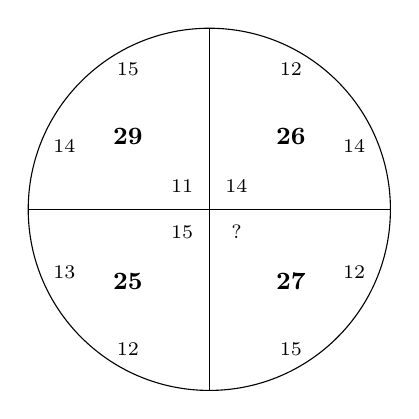
\begin{tikzpicture}[scale=1.15,font=\scriptsize]
\draw (0,0) circle(2); \draw (-2,0)--(2,0); \draw (0,-2)--(0,2);
\node at (-0.9,1.55){15}; \node at (-1.6,0.7){14}; \node[font=\small\bfseries] at (-0.9,0.8){29}; \node at (-0.3,0.25){11};
\node at (0.9,1.55){12}; \node at (1.6,0.7){14}; \node[font=\small\bfseries] at (0.9,0.8){26}; \node at (0.3,0.25){14};
\node at (-1.6,-0.7){13}; \node at (-0.9,-1.55){12}; \node[font=\small\bfseries] at (-0.9,-0.8){25}; \node at (-0.3,-0.25){15};
\node at (1.6,-0.7){12}; \node at (0.9,-1.55){15}; \node[font=\small\bfseries] at (0.9,-0.8){27}; \node at (0.3,-0.25){?};
\end{tikzpicture}

%% Q41
In each quadrant the centre number is the sum of the two outer numbers, and the inner (corner) number is $40-$ centre:
\begin{center}\small
\begin{tabular}{lccc}\toprule Quadrant & Outer sum & Centre & Inner $=40-$centre\\\midrule
Top-left & $15+14$ & 29 & 11\\ Top-right & $12+14$ & 26 & 14\\ Bottom-left & $13+12$ & 25 & 15\\ Bottom-right & $12+15$ & 27 & \textbf{13}\\\bottomrule
\end{tabular}
\end{center}

%% Q42
Each letter moves two steps back: U$\rightarrow$S, P$\rightarrow$N, E$\rightarrow$C. So QHD $\rightarrow$ \textbf{OFB}.

%% Q43
Attachments from unknown senders may carry \textbf{viruses or malware} (executables, macros) that infect the computer when opened.

%% Q44
The top-level domain \texttt{.org} denotes an \textbf{organisation}, typically a non-profit. (\texttt{.com} = commercial, \texttt{.edu} = education, \texttt{.gov} = government.)

%% Q45
\textbf{URL} is \textbf{Uniform Resource Locator}.

%% Q46
In a democratic institution, communication is predominantly \textbf{horizontal}: among peers and equals, participative and consultative, rather than top-down.

%% Q47
Word, Excel and Access are \emph{application software} (MS Office). \textbf{Windows} is an \emph{operating system}, so it is the odd one out.

%% Q48
\textbf{Terabyte} is the largest: TB $>$ GB $>$ MB $>$ KB.

%% Q49
In big Indian cities, \textbf{vehicular traffic} is the dominant source of air pollution (NO$_x$, CO, particulate matter), especially at ground level where people breathe.

%% Q50
Vegetables, bones and earthworms are organic and are decomposed by microbes. \textbf{Iron rust} (hydrated iron oxide) is inorganic and not biodegradable.

%% Q51
Global warming is expected to cause loss of deltas (sea-level rise), changed precipitation and more intense hurricanes. Higher CO$_2$ tends to \emph{increase} photosynthesis (the CO$_2$ fertilisation effect), so a \textbf{decreased rate of photosynthesis} is the least likely effect.

%% Q52
The ``lead'' of a pencil is \textbf{graphite} (a form of carbon) mixed with clay. Pencils contain no lead.

%% Q53
Most tsunamis are generated by undersea \textbf{earthquakes} (sudden displacement of the sea floor), e.g.\ the 2004 Indian Ocean tsunami (magnitude 9.1).

%% Q54
The \textbf{Sardar Sarovar} dam is on the \textbf{Narmada} river at Kevadia (Ekta Nagar), Gujarat, near the Statue of Unity.

%% Q55
\textbf{RUSA} (2013) aims at improving access, equity and quality in state higher education. Its basic concern is to raise \textbf{GER, i.e.\ to overcome low enrolment} in higher education (target 32\% by the end of the 12th Plan).

%% Q56 note
Under the approved RUSA scheme the Centre--State ratio was 65:35 for general-category states (90:10 for special-category states). The official key nevertheless gives (A).

%% Q56
The official key gives \textbf{75\% Centre : 25\% State}, the funding pattern cited in early RUSA documents. RUSA funds reach state universities and colleges through state higher-education councils.

%% Q57
In higher-education policy, \textbf{PPP} means \textbf{Public--Private Partnership}: collaboration between government and private players to expand and improve institutions.

%% Q58
UGC introduced the \textbf{NET} (1989) as the minimum eligibility for Assistant Professors to \textbf{ensure merit and uniform standards in the recruitment of teachers}.

%% Q59
GER $=$ enrolment of \emph{all ages} in a level $\div$ population of the official age group. Because \textbf{repeaters and under- or over-age students} are counted in the numerator, GER can exceed 100.

%% Q60
Governance of higher education faces the challenge of \textbf{meeting funding requirements}: institutional finance, autonomy linked to funding, and efficient use of resources.
